\documentclass[letterpaper]{article}

\usepackage{amsmath, hyperref, enumerate}
\usepackage{amsfonts}
\usepackage{graphicx}

\usepackage[backend=biber,  style=chicago-authordate, url=false, doi=false, eprint=false]{biblatex}
%\usepackage[backend=biber,  style=authoryear-icomp, url=false, doi=false, eprint=false]{biblatex}
\addbibresource{bibliography.bib}

\AtEveryBibitem{%
  \clearfield{note}%
  \clearfield{series}%
  \clearfield{pages}%
}



\begin{document}

%% testing from desktop

\title{TBD}
\author{TBD}

\date{\today}

\maketitle

\begin{abstract}
	TBD
\end{abstract}


Current section ideas:

\begin{enumerate}[1.)]

\item Assumptions of physics framework section

\begin{itemize}

\item motivate everything upfront: going to show that Hamiltonian mechanics corresponds to two conditions being satisfied, while Lagrangian mechanics requires a three condition
\item define the two assumptions, and give motivation
\item figuring out which mathematical structures are required for systems that satisfy certain physical conditions
\item go over the upshot of the philosophical argument, specifically how this avoids the worries about measuring the amount of structure that plagued North (i.e. Swanson and Halvorson paper)
\item Then, give the derivation, as gentle and well-motivated as possible. But would be ideal if readers could skip or skim this section and still get the philosophical upshot, relatively early on.

\end{itemize}

\item Physical significance of invariant distributions

\begin{itemize}

\item explain how these provide a novel way of understanding things, one that we can physically privilege

\item connect this with North on invariant structure, but disavow metaphysical commitments


\end{itemize}

\item How to interpret Lagrangian mechanics in light of Hamiltonian mechanics

\begin{itemize}

\item gauge transformation stuff
\item go over the cool stationary action principle derivation/argument
\item clarify the status of Riemannian metric structure in the Lagrangian formalism
\item respond to Curiel's privileging of Lagrangian mechanics
\item respond to Curiel's argument that Hamiltonian mechanics involves the imposition of an ad hoc condition in order to get the right kinematical constraints, whereas these fall out naturally from Lagrangian mechanics.


\end{itemize}

\item Considerations in light of categorical equivalence proofs

\begin{itemize}

\item  clarify that argument is not in tension with categorical equivalence within the hyper regular domain. make this precise.
\item Respond to the worry that something must have gone amiss if we have a difference in the number of conditions required for the Hamiltonian vs. Lagrangian mechanics, yet still have categorical equivalence in the hyper-regular domain

\end{itemize}

\end{enumerate}

\section{Introduction}

TODO: Lagrangian assumption vs kinematic assumption. Investigate what happens when the transformation is non-linear.

Philosophers have recently shown that we can interpret Lagrangian and Hamiltonian mechanics as theoretically equivalent in a precise mathematical sense. Within a subclass of classical mechanical systems known as the \textit{hyper-regular domain}, the two formalisms are categorically equivalent \parencites[]{Teh2017}{Barrett2018}. Categorical equivalence provides a natural interpretive criterion for theoretical equivalence because it yields mutual inter-translatability between theory formulations. At first glance, this equivalence seems to motivate the view that there are no physically significant differences between these two formalisms, at least within the hyper-regular domain. This view would undermine prior debates that have privileged either Hamiltonian mechanics or Lagrangian mechanics on physical or metaphysical grounds \parencites[]{North2009}{Curiel2014}. Here, we will argue that there are indeed physical grounds for privileging Hamiltonian mechanics over Lagrangian mechanics, their categorical equivalence notwithstanding. Compared to Hamiltonian systems, an additional physical condition must be satisfied for a classical system to be Lagrangian. Hamiltonian mechanics thereby captures a wider range of systems than Lagrangian mechanics, and this conceptual difference has interpretive consequences even within the hyper-regular domain. Furthermore, the construction at the heart of this argument provides an interpretation of classical mechanical systems in terms of their invariant phase space density, along with a novel interpretation of the principle of stationary action within the Hamiltonian formalism.

Thesis: despite the mathematical equivalence of Hamiltonian and Lagrangian mechanics within the hyper-regular domain, the two frameworks have important differences. In particular, Hamiltonian systems arise when a smaller number of basic physical conditions are met. A Lagrangian system must satisfy a further physical condition. This shows that Hamiltonian mechanics is in a sense more fundamental. Defending this claim does not require commitments to fundamental structure or perfectly natural properties.

Targets: Curiel's privileging of Lagrangian mechanics and argument that Hamiltonian mechanics is ad hoc; North's somewhat flawed privileging of Hamiltonian mechanics on the basis of it requiring less structure; a motivation stemming from categorical equivalence proofs for thinking that there are no physically significant differences between the Hamiltonian and Lagrangian frameworks (at least within the hyper regular domain).

Goals: provide a gentle introduction to Assumptions of Physics framework, and show that it has real philosophical payoffs for interpreting physical theories, such as classical mechanics.



\subsection{Define Classical Mechanics}

Talk about dissipative systems.

Throughout, we will focus only on non-dissipative classical systems, i.e. conservative systems. For in the context of transforming between the Hamiltonian and Lagrangian formulations (via a Legendre transform), we assume that the conjugate momentum $p$ is the derivative of the Lagrangian with respect to the generalized velocity $v $. This requires that the system is conservative [why exactly?], which is equivalent to the system being deterministic and reversible. Consequently, we will not consider systems that satisfy inhomogenous Euler--Lagrange equations.
% Dissipative systems contain more information than contained in the Lagrangian alone, namely, the additional information contained in the Rayleigh potential

\subsection{Derivation}

\begin{figure}[h]
	\centering
	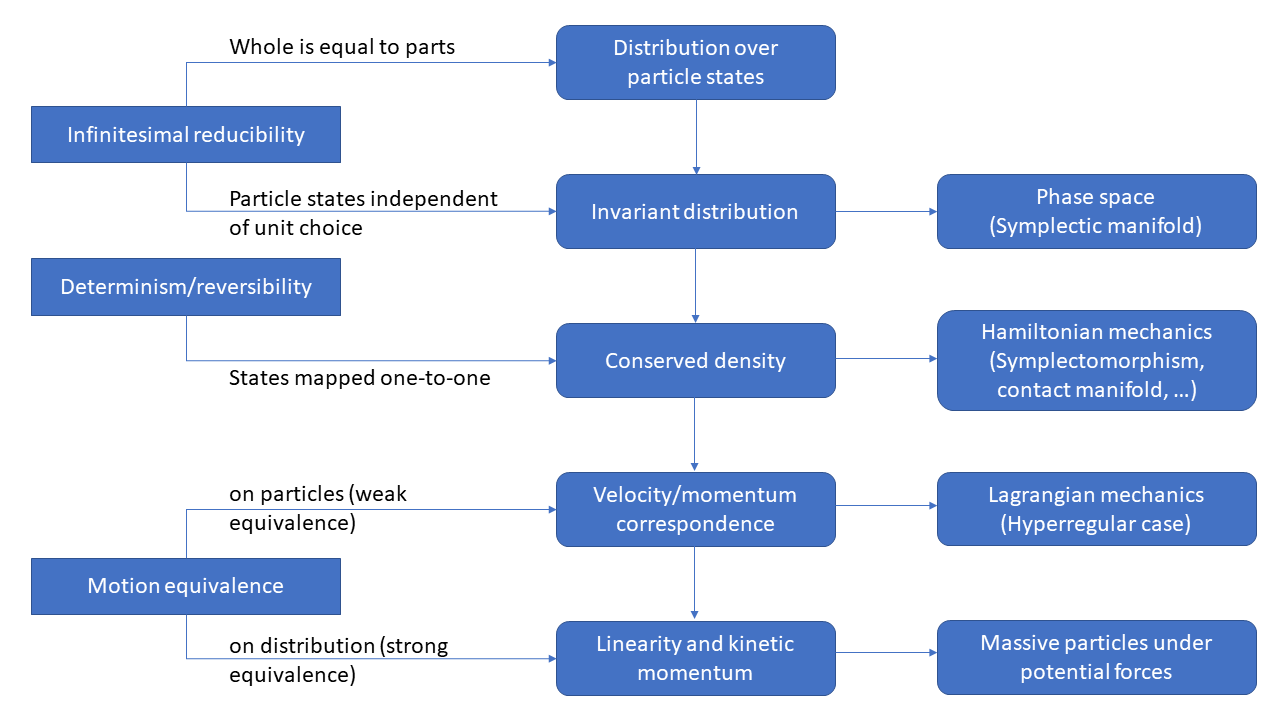
\includegraphics[width=\textwidth]{Diagram.png}
\end{figure}

Overall summary: A classical system is an infinitesimally reducible system. The state space of these systems can be modeled by a symplectic manifold (the physical assumption of infinitesimal reducibility corresponds to the mathematical structure of symplectic manifolds). Classical Hamiltonian systems satisfy the additional conditions of having deterministic and reversible evolutions. These two physical assumptions entail the existence of a symplectic morphism on the state space manifold, making it a contact manifold. Classical Lagrangian systems satisfy a further assumption: keeping track of the trajectories in physical space is equivalent to tracking the evolution of states in phase space. Note that it is not always true that we can determine the evolution in phase space from the trajectory in physical space. For instance, knowledge of the trajectory of a photon is insufficient for knowledge of its phase space evolution, since we cannot determine the momentum of a photon from its trajectory alone. Hence, the set of classical systems that satisfy this further physical condition is a proper subset of the classical systems that satisfy the assumptions for Hamiltonian mechanics.

\subsubsection{Infinitesimal reducibility}

First, we will show that a classical phase space arises if and only if a system satisfies the following physical condition:

\begin{quotation}
Infinitesimal reducibility assumption: the state of the system is reducible to the state of its infinitesimal parts. That is, giving the state of the whole system is equivalent to giving the state of its parts, which is equivalent to giving the states of those parts, and so on.
\end{quotation}

\noindent
This assumption characterizes classical systems as those whose infinitesimal parts completely specify the state of the system. [At least in a footnote: comment on how this characterization of infinitesimal particles relates to standard philosophy of physics interpretive disputes over the status of point particles in classical mechanics. See Butterfield Pointillisme article; Butterfield characterizes particles as extensionless.]

Let $\mathcal{C}$ be the state space for the whole system. Any point $c \in \mathcal{C}$ represents a particular state of the whole system. We define a classical \textit{particle} as the limit of recursive subdivision. A classical system then consists of a collection of classical particles. Let $\mathcal{S}$ be the state space for the particles [all of the particles constituting the whole system? or for each particle individually?]. We assume that this state space $\mathcal{S}$ is a manifold. Then for each state $c \in \mathcal{C}$ there exists a unique distribution $\rho_c : \mathcal{S} \to \mathbb{R} $ that describes the state of $c$'s parts. That is, the state of the whole system is a distribution over its infinitesimal parts. If $\mathcal{S}$ is a manifold, $\int_U \rho_c d\mathcal{S}$ gives us the fraction of the system whose parts are in the region $U$ of the state space $\mathcal{S}$. 
%[is region U in the state space C or S. I assume in S.].

On physical grounds, the distribution $\rho_c$ must transform as both a density and a scalar function, i.e. it must depend on the point [the point $c $? ] and not on the coordinates. This is because the distribution is a function only of the states, rather than of the particular choice of state variables, i.e. coordinates. [Explain why these two physical conditions hold for the distribution. Also, explain what it means to transform as a density.] We will now show that classical phase space (i.e. a symplectic manifold) is the only space that satisfies these constraints on the distribution. 

We define the \textit{state variables} as a set of quantities $\xi^a$ that fully identify a state (in manifold terminology, these are known as coordinates). We will define a \textit{coordinate} $q \in \xi^a$ as a particular state variable that defines a unit. For instance, $q$ might be position, defining units of meters. Starting with the simplest case, suppose that one coordinate suffices to define the unit system for the particle state space. Then, the state variables are given by a set $\xi^a = \{ q, k^i \}$, where \textit{prima facie} the index $i$ can range over more than one number. We will show that, in fact, there can only be a single $k^i$ coordinate in this case, conjugate to the single $q$ coordinate. Our derivation assumes---on physical grounds---that we can (i) arbitrarily change the unit defined by $q$ without changing the density $\rho_c$ and that (ii) $q$ fully defines the units for all state variables. 
%[Give a concrete example of a state variable defining a unit, along with physical motivation for why state variables play the role of defining units (since we are treating this as a physically grounded assumption).]
% How many $k^i$ can we have?

[We need to introduce the definition of state variable evolution $s$, since we appeal to it below. I take it that the definition we are working with is that future states are labeled by the original state variable values (i.e. transported state variables)? Section IV.C of long paper.]

Now, suppose that we change the units by transforming the coordinate $q$ to a new coordinate $\hat{q}$ that is a function of the old coordinate: $\hat{q}=\hat{q}(q)$. Call the new units $\hat{\xi}^b = \{ \hat{q}, \hat{k}^i\}$. We have $\rho_c(\hat{\xi}^b)=\rho_c(s(\hat{\xi}^b))=\rho_c(s(\xi^a))=\rho_c(\xi^a) = \left|\frac{\partial \hat{\xi}^b}{\partial \xi^a} \right| \rho_c(\hat\xi^b)$. Therefore the Jacobian $\left|\frac{\partial \hat{\xi}^b}{\partial \xi^a} \right|$ must be equal to 1. Suppose there is only one state variable, so that there are no $k^i$ variables. Then we would have $\left|\frac{\partial \hat{\xi}^b}{\partial \xi^a} \right| = \left|\frac{\partial \hat q}{\partial q} \right| = 1$. But this would mean the unit change cannot be arbitrary. Therefore we must have two or more variables, so that there is at least one $k^i$ variable. The requirement that the Jacobian determinant equals one places a constraint on how the state variables $k^i$ must change to compensate the change from $q$ to $\hat q$. Note that, since $\hat{q}$ depends only on $q$, the Jacobian is an upper triangular block matrix, so $\left|\frac{\partial \hat{\xi}^b}{\partial \xi^a} \right| = \left|\frac{\partial \hat q}{\partial q} \right|\left|\frac{\partial \hat{k}^b}{\partial k^a} \right|$ [it might be worthwhile to spell this out in more detail].  For the Jacobian determinant to equal one, we must therefore have $\left|\frac{\partial \hat{k}^b}{\partial k^a} \right| = \left|\frac{\partial q}{\partial \hat q} \right|$. This places a constraint only on the determinant of the transformation. Suppose there are three or more variables. This constraint would then be insufficient to recover the transformation uniquely, and therefore $\hat q$  would not fully define the units for all other state variables (contrary to assumption). This means there must be exactly two state variables: $q$ and a single $k$. So in this case, coordinate-independent areas and densities can only be defined on a two-dimensional manifold.

To generalize, we say two coordinates are \textit{independent} if changing the units for one does not change the units for the other. Suppose our particle state space $\mathcal{S}$ is such that its units are fully defined by $n$ independent coordinates $q^i$. Suppose you change the first coordinate $q^1$ without changing the others. Then we will find a variable $k_1$ that changes as before so that the densities are invariant. Now change the second coordinate $q^2$ in the same way while also fixing $k_1$. Then we find a corresponding $k_2$. In the end, we will find that $\mathcal{S}$ is $2n$-dimensional, and the state variables are $\xi^a = \{ q^i, k_i \}$. We define an \textit{independent degree of freedom} as the space charted by a pair of such variables.

We can now show that $\mathcal{S}$ is a symplectic manifold. Invariant densities can only be assigned to infinitesimal areas. Therefore we need a two-form $\omega$ that assigns an infinitesimal area to each infinitesimal surface, so that we can define integrals of the form $\int_{\Sigma} \rho_c \omega(d\Sigma)$ [clarify which phase space $\Sigma$ belongs to]. Because degrees of freedom are---at least locally---independent, the total number of states in a volume is the product of the possible configurations of each degree of freedom. This means the volume form is given by $\omega^n$. This cannot be degenerate, or some volumes would not contain states [motivate this claim or]. Therefore $\omega$ itself cannot be degenerate. As the degrees of freedom are independent, the number of states on a surface does not change if we translate it across independent degrees of freedom. If we imagine a parallelepiped, the integral over the surface must be zero (the integrals over opposite sides are equal and opposite). Therefore $\mathcal{S}$ must come equipped with a two-form $\omega$ that is closed and not degenerate, and therefore $\mathcal{S}$ is a symplectic manifold. By convention, we set $\omega = \hbar dq^i \wedge dk_i = dq^i \wedge dp_i$ where $p_i = \hbar k_i$.

The conclusion is that, under the infinitesimal reducibility assumption, the state space of the system is a coordinate-invariant distribution over the state space of the infinitesimal parts [what does it mean for the state space $\mathcal{C} $ to itself be a distribution ?]. If the state space of the particles is a manifold, then it is a symplectic manifold, which is the only type of manifold that supports coordinate-invariant distributions [do we have a reference to substantiate the ``only" claim? Has the proof above really shown that this is the only kind of manifold that would support a coordinate-invariant distribution].

\subsubsection{Deterministic and reversible evolution}

Next, we assume that the classical systems of interest are deterministic and reversible. This amounts to satisfying the following joint condition:

\begin{quotation}

Deterministic and reversible evolution assumption: given the present state of the system, all future (determinism) and past (reversible) states are uniquely identified.

\end{quotation}

[Should we footnote that these two assumptions leave out some classical systems, e.g. Norton's dome, Earman's space invaders?]

In our case, this applies to both the state of the whole system and to the state of its parts. Let $\lambda : \mathbb{R} \to \mathcal{S}$ be the evolution over time of the state of a particle. Under the assumption, this will be uniquely identified by the initial state $s_0 = \lambda(t_0)$ at the initial time $t_0$. [is $s$ an evolution that transports the state variables, i.e. labeling future states by the original state variables so that the initial time is transported to itself? I think we need to explain more about how evolutions are defined]. Moreover, if $\rho(\lambda(t_0), t_0)$ is the density associated to the initial particle [what exactly does `initial particle' mean? Do we mean the initial state of the composite system or just a particular particle?] at the initial time, we must have that $\rho(\lambda(t), t) = \rho(\lambda(t_0), t_0)$, i.e. the density remains the same throughout the evolution. In other words, all particles that begin in a given initial state must end up in the same final state and vice-versa [could two different particles occupy the same initial state?].

Now consider the integral $\int_{\Sigma} \rho_c \omega(d\Sigma)$. The region $\Sigma$ will be mapped to a new region, but the fraction of the system found in both the old and new regions must be the same. Since both the integral and $\rho_c$ must remain constant during the evolution, the two-form $\omega$ must also remain the same. That is, the areas in phase space must be mapped to areas of equal size, and independent degrees of freedom must be mapped to independent degrees of freedom (otherwise, volumes would not be mapped to equal volumes, which would violate determinism). The evolution is a symplectomorphism and corresponds to Hamiltonian evolution. Intuitively, this argument is the inverse of Liouville's theorem: instead of positing Hamiltonian evolution and finding conservation of areas and volumes, deterministic and reversible evolution imposes the conservation of areas and volumes which leads to Hamiltonian evolution.


\subsubsection{Motion equivalence}

Having recovered classical Hamiltonian mechanics, the laws of evolution become further restricted when the following condition holds:

Motion equivalence assumption: the motion of the system (i.e. trajectories in physical space-time) is enough to recover its dynamics (i.e. evolutions in state space) and vice-versa.

If we focus on the parts of the system, this means that for every evolution in phase space there should be one and only one trajectory in physical space. Note that each space variable $x^i$ is a coordinate, i.e. a state variable that defines a unit. In fact, the trajectories can be fully described by these units and only these units. So we can say that $q^i=x^i$, each $q^i$ will be paired with a conjugate $p_i$ and each state $\{q^i, p_i\}$ will be mapped to one and only one trajectory. At each point $x^i$, then, infinitely many trajectories must pass, one for each combination of $\{p_i\}$. Since the trajectories are differentiable in $x^i$, we can define a velocity $v^i = d_t x^i$. If the equations of motions were such that $v^i=v^i(q^i)$, then motion equivalence would fail as the full trajectory would be determined only by the $q^i$. So we must have $v^i=v^i(q^i, p_i)$. This relationship must be invertible or motion equivalence would fail. At any given time, then, we must have the following relationships:
\begin{equation}
\begin{aligned}
x^i &= q^i \\
v^i &= d_t x^i = v^i(q^j, p_k)
\end{aligned}
\end{equation}

In this case, which we call \textit{weak equivalence}, $v^i(q^j, p_k)$ must be invertible at every $q^i$. Therefore, the Jacobian matrix  $\frac{\partial v^i}{\partial p_j}$ must be invertible. Since $v^i = d_t q^i = \frac{\partial H}{\partial p_i}$, the Hessian $\frac{\partial^2 H}{\partial p_i \partial p_j}$ must be non-zero everywhere, and therefore must have the same sign which we take to be positive. These are exactly the cases where a Lagrangian can be constructed, and where the Lagrangian leads to a unique solution (via the stationary action principle).

If we look at the whole distribution, we have $\rho(q^i, p_j) = |J| \rho(x^i, v^j) = \left|\frac{\partial v^i}{\partial p_j}\right| \rho(x^i, v^j)$ since
\begin{equation}
\begin{aligned}
|J| &= \begin{vmatrix}
\frac{\partial x^i}{\partial q^j} & \frac{\partial x^i}{\partial p_j} \\
\frac{\partial v^i}{\partial q^j} & \frac{\partial v^i}{\partial p_j}
\end{vmatrix}
= \begin{vmatrix}
\delta^i_j & 0 \\
\frac{\partial v^i}{\partial q^j} & \frac{\partial v^i}{\partial p_j}
\end{vmatrix} \\
&= \left|\delta^i_j\right| \left|\frac{\partial v^i}{\partial p_j}\right| - \left|0\right| \left|\frac{\partial v^i}{\partial q^j}\right|
= \left|\frac{\partial v^i}{\partial p_j}\right|.
\end{aligned}
\end{equation}
Note that while the value given by $\rho(q^i, p_j)$ is coordinate independent, the value given by $\rho(x^i, v^j)$ depends on the choice of coordinate through $\left|\frac{\partial v^i}{\partial p_j}\right|$. If $x^i$ truly sets the unit system by itself, then $\left|\frac{\partial v^i}{\partial p_j}\right|$ must be a function of position only. Similar considerations will also hold for marginal distributions (i.e. distributions on a subset of the coordinates) which means all components of $\frac{\partial v^i}{\partial p_j}$ must be a function of position only. We set:
\begin{equation}
\begin{aligned}
\frac{\partial v^i}{\partial p_j} = \frac{1}{m} g^{ij} \\
\frac{\partial p_j}{\partial v^i} = m g_{ji}
\end{aligned}
\end{equation}
where $m$ is the unit conversion constant between velocity and conjugate momentum while $g_{ij}$ represents the linear dependency.

If we integrate, we have:
\begin{equation}
\begin{aligned}
v^i = \frac{1}{m} g^{ij}(p_j - A_j) \\
p_j = m g_{ji} v^i + A_j
\end{aligned}
\end{equation}
where $A_j$ are arbitrary functions. Note that:
\begin{equation}
v^i = d_t q^i = \frac{\partial H }{\partial p_i} = \frac{1}{m} g^{ij}(p_j - A_j) \\
\end{equation}
We integrate yet again and find:
\begin{equation}
H = \frac{1}{2m} (p_j - A_j) g^{ij}(p_j - A_j) + V \\
\end{equation}
where V is another arbitrary function. We recognize this as the Hamiltonian for massive particles under potential forces.

[Connect this with Curiel equation 6.2 for the Hamiltonian.]





\section{Argument for privileging Hamiltonian mechanics}

\subsection{Relevant formal background from assumptions of physics framework}

%On the notion of more or less structure, treated in such a way that we avoid the objections of Halvorson/Swanson against North's notion of amount of structure:
Our comparisons of structure arise from logical chains of strict entailment, wherein something has more structure if and only if it is less general, i.e. if and only if it is a specialization of a more general case. So in this case, the Lagrangian framework has more structure than the Hamiltonian framework because Lagrangian mechanics requires an additional assumption. This difference in the number of assumptions corresponds to a difference in the number of commitments. When working with a Hamiltonian but non-Lagrangian structure, we are not committed to the q's being positions (although is this in tension with the remarks on the significance of the coordinate and unit systems?). In contrast, for systems where motion equivalence applies, we gain the further commitment of treating the q's as positions.

Hamiltonian mechanics makes fewer assumptions on the physical system being studied than Lagrangian mechanics. Lagrangian is a subset than Hamiltonian. Makes ``amount of structure" more rigorous. Hamiltonian defines the relationship between conjugate momentum and velocity ($dq/dt = \partial H / \partial p$), so kinematic assumption constrains the Hamiltonian.


Claim to think about: GC was arguing on 10-12 that you could handle classical systems in the Hamiltonian framework with just a differential manifold and no symplectic structure. This would contradict North's indispensability claim that Hamiltonian symplectic structure is necessary for treating classical systems. E.g., North footnote 31: ``The symplectic form is crucial to determining the motion, since the same Hamiltonian can induce different flows for different symplectic forms" [76]. North takes this as an argument for why we cannot eliminate the symplectic form in an attempt to get at even less structure. We need it to define the dynamics.

\subsection{The significance of invariant distributions}

North argues that Hamiltonian mechanics is superior because it requires strictly less structure than Lagrangian mechanics. While we agree that Hamiltonian mechanics does require less structure---in a different sense than North's account---this is not the only grounds for privileging it. Instead, the main grounds for privileging Hamiltonian mechanics comes from understanding physics in terms of invariant distributions. This allows us to provide a better physical interpretation of the action principle, which holds even when a Lagrangian cannot be defined for the system of interest.
% Do we agree with the following claim defended by North: ``as far as we can tell, we need only symplectic structure to do classical mechanics" [74]. 

Hamiltonian mechanics is ``fundamental" because allows to show that densities are coordinate independent quantities and therefore physical quantities. Canonical pairs (position and conjugate momentum) allows a simpler expression/comparison of densities over space. That is why statistical mechanics works best on phase space (we have a uniform measure over q/p).

Can characterize this argument as physically or epistemically privileging Hamiltonian mechanics 

\subsection{Response to Curiel's criticisms of Hamiltonian mechanics}



Curiel restricts Hamiltonian mechanics to systems whose Hamiltonian takes the form (equation 6.2) $H =\alpha^{m n} p_m p_n + U (q_j) $. Here, the functions $U$ and $\alpha^{m n}$ are arbitrary functions of the generalized position coordinates $q $. Curiel's argument in a nutshell:  ``Hamiltonian mechanics represents abstract classical systems only in so far as we restrict ourselves to a subfamily of all the formally acceptable Hamiltonians by the \textit{ad hoc} use of conditions foreign to Hamiltonian mechanics itself. Its structures do not provide the appropriate concepts and tools to formulate in their terms the required structures that treat configurative quantities differently from momental, nor do they provide any natural justification for the restriction to Hamiltonians of the form (6.2)" (306). 

Curiel argues that Hamiltonian mechanics is less physically significant than Lagrangian mechanics. His argument hinges on the claim that Hamiltonian mechanics requires an ad hoc condition that is imposed by hand, whereas Lagrangian mechanics follows from physically plausible principles. We agree with Curiel that his equation 6.2 requires a condition that is imposed by hand, namely the kinematic equivalence assumption. However, this condition has a clear physical meaning, and it corresponds to a physical condition that must hold in order to define/apply Lagrangian mechanics. Pace Curiel, there exist Hamiltonian systems that do not satisfy his equation 6.2 (equivalently, classical systems where the momentum is not a linear function of the velocity), and these will even have a Lagrangian, although they will not be an abstract classical system in Curiel's sense. Hence, there seems to be a burden on Curiel to distinguish---in a principled way---the classical Lagrangian systems from those that are not classical.
% Hence, perhaps we agree with Curiel that ``it is not necessary that [these conditions] hold in order for the theory to be meaningfully applied to model a [classical] system" [305]. Where is Curiel takes this as an argument for the primacy of Lagrangian mechanics, we take it as an argument for the primacy of Hamiltonian mechanics, since Curiel's conditions are equivalent to imposing motion equivalence.

Response: symplectic geometry indeed does not care about the difference between q's and p's. Classical mechanics does. Misindentification of the math (symplectic geometry) with the physics (Classical Hamiltonian mechanics).

Curiel's main point: the representation of a classical mechanical system in the Lagrangian framework is \textit{natural} in a way that its representation in a Hamiltonian formulation is not. The former representation depends on intrinsic structures of the classical mechanical system rather than an artificial construction (270).

Part of our response: The action principle can be understood geometrically in the extended phase space as a consequence of ``state density" conservation. It also holds when the action cannot be expressed as a function of just position and velocity, since it can always be expressed as a function of position and conjugate momentum. Also shows that Lagrangian is ``unphysical" and depends on gauge.


Upshot: can better understand Lagrangian mechanics as a special case of Hamiltonian mechanics. Explain how the geometrical understanding of the stationary action in extended phase space should meet any criterion of ``naturalness" or ``natural construction." Lagrangian mechanics is actually less natural because contingent on having a bijection between velocity and conjugate momentum.

On its own, the kinematic/motion of a system in physical space is not sufficient for defining the system's dynamics. The kinematics/motion does not suffice to determine the forces acting on the system. For it is essential to be able to distinguish the forces acting on an inertial system from fictitious forces arising in the description of a non-inertial system. Hence, unless one knows that the kinematic equivalence principle is satisfied, Lagrangian mechanics faces an underdetermination problem: it is unable to distinguish between certain inertial vs. non-inertial systems that are physically distinct. Distinguishing between these kinds of systems requires a relationship between conjugate momentum and kinematic momentum (or equivalently, knowledge of the energy/Hamiltonian).
% Example of underdetermination in the context of Lagrangian mechanics: a free particle in a non-inertial frame vs. an accelerated particle (in an inertial frame) acted on by a dissipative force. These two distinct classical systems can nevertheless have the same equations of motion.
% The Hamiltonian framework does not face a corresponding underdetermination problem because it does not allow for dissipative systems. Hence, there is a sense in which the Lagrangian formalism is more mathematically general than the Hamiltonian formalism. However, this additional generality is irrelevant when considering conservative classical systems.

The standard predator--prey model from differential equations satisfies Curiel's definition of an abstract classical system. However, it does not satisfy Curiel's notion of the split between configurational vs. velocital coordinates. And it is not true that the velocity will be the first derivative of the position. Moreover, the predator--prey system is neither Hamiltonian nor Lagrangian, because it is not necessarily deterministic and reversible.
% Related to equation 3.1. Make precise.
% Furthermore, the momentum does not need to be a linear function of velocity. For example, the photon does not satisfy this relationship.

Objection against Curiel to make precise and substantiate with textual evidence: implicitly, Curiel assumes that classical systems are defined as Newtonian systems in an inertial frame with Cartesian coordinates. Implicitly, Curiel assumes that energy is a function of position and velocity, entailing that we have a Hamiltonian. The claim in footnote 17 that the kinetic energy is a function of velocity depends on the choice of a particular coordinate system; it is not a coordinate-invariant claim. Curiel's thought experiment assumes that we have a constant force (in this case gravity) and that we are in a reference frame where we can compare forces (e.g. an inertial frame).

\subsection{Discussion of relation to categorical equivalence proofs}

Possible objection to consider stemming from categorical equivalence: for systems in the hyper regular domain, does the categorical equivalence of Hamiltonian and Lagrangian mechanics show that we require the same number of assumptions to treat systems in this domain? 
Some relevant considerations for responding: note that the photon does not belong to the hyper regular domain. Furthermore, if you are not in the hyper regular domain, then there is no longer a one-to-one map between position and velocity. In this sense, the Hamiltonian framework is more general because it applies outside the hyper regular domain: the Hamiltonian can define a unique solution (unique evolution in phase space) even when the Hessian is zero. In contrast, whenever the Lagrangian is not hyper regular, the Euler--Lagrange equations do not possess a unique solution. Furthermore, density plays a special role in the Hamiltonian framework, whereas it is in some sense an accident that the density and configuration space is invariant (simply because the Jacobian equals unity in Cartesian coordinates).

\section{A non-metaphysical notion of fundamentality}

%Different notions of fundamentality, perfectly natural properties, naturalness, etc. 

%Joint carving, perfectly natural properties. Ontological notion of fundamental. Clearly state why this is not ``good" for this context. We are agnostic. One may use following points to argue whatever they want.

Whereas North \parencites*[76]{North2009} seeks to determine the `real' fundamental state space structure of the theory---and correspondingly, of a classical world---we remain neutral on this underlying metaphysical question. Whether Hamiltonian phase space structure is metaphysically fundamental is neither here nor there for the questions we seek to answer. For regardless of its metaphysical status, Hamiltonian mechanics is epistemically, conceptually, and physically more fundamental.
% Similarly, Curiel advocates neutrality on these metaphysical issues when it comes to the conceptual analysis of a physical theory's structure (304).
% On the basis of the fundamentality of Hamiltonian mechanics, North argues that ``we should infer that symplectic structure is the `real' state space structure of the theory. We should infer that this structure corresponds to the `real' physical structure of a classical mechanical world" [76]
%``there is an objective fact about what structure exists, there is a privileged carving of nature at its joints: along the lines of its fundamental physical structure" [82]. 

Methodologically, we agree with North that it is important to identify invariants and more generally ``the mathematical structure needed to formulate the theory in an invariant, frame-independent way" \parencites*[65]{North2009}. Additionally, we agree that it is worthwhile to identify what particular mathematical structure is required by a formulation \parencites[78]{North2009}. However, whereas North proceeds mainly from the mathematical structure to claims about physical significance, we seek to interpret the mathematics by beginning with physically significant assumptions. We seek to determine which physical assumptions are necessary and sufficient for supporting a corresponding mathematical structure. This does not entail that additional mathematical structure is necessarily physically insignificant or surplus structure, just that it may correspond to an additional physically significant assumption that might apply to the system under consideration. As we will see, this characterizes the relationship between Hamiltonian and Lagrangian formalizations of a classical system. Hence, whereas North views the Lagrangian structure as surplus or redundant (``excess, superfluous structure"), we take the Lagrangian structure as unnecessary but still physically significant, corresponding to an additional physical assumption that applies to some classical systems.
% % Similarly, we agree with the general methodology of Curiel as well: ``One task of the philosopher of physics is to work out the conceptual structure of a physical theory---or at least an appropriate one, if it is not unique---to isolate and characterize its mathematical and formal structures, and show how natural physical interpretation accrues to them from an analysis of their empirical application" (272).
% I think that Curiel might make a similar point regarding the significance of a formulation even if it uses surplus structure or less physically significant structure. See section 7 argument against structural realism: Curiel argues that the Hamiltonian formulation nevertheless does not fail to represent classical systems, even if it structure is not the most natural (on his view)
%having argued that Lagrangian mechanics has more structure ``than the theory really needs", North claims that ``we should infer that it does not exist, that it does not correspond to fundamental structure" [75]. 
% Curiel on the harmonic oscillator: claims to have given an example where there is sameness of meaning (both Lagrangian and Hamiltonian formulations represent the harmonic oscillator and provide the same meaning) without sameness of structure (they're not isomorphic).
%``we should infer that the world contains at least the amount of structure needed to formulate its fundamental dynamics in an invariant way" [80].
% E.g., North argues that ``only certain kinds of mathematical object are appropriate for representing the structure of the world" and it is through these facts that we figure out which formulation of physics to prefer? [66].


We agree that providing a physical interpretation of the invariants is important. However, some non-invariant quantities can be physically meaningful. For instance, the coordinates q define the units, and these are physically significant despite not being invariant. Units are physically significant because they allow us to assign numbers to a physical quantity. They are physically significant in part because they correspond to measurable quantities. Whereas North claims that coordinate choices are ``merely arbitrary choices of description" \parencites*[61]{North2009}, some choices of the coordinates q are less physically meaningful because they are not properly connected with measurement. Some arbitrary mixings of q's and p's preserve the symplectic manifold but are not as physically significant. For this reason, the q's are epistemically privileged because they are linked with measurements, in a sense that the logically-derivative p's are not. The p's are inverses of the q's. Whereas symplectic geometry creates a mathematical, syntactic symmetry between the q and p variables, this is not a physically significant symmetry from the standpoint of measurement.
Moreover: could discuss how Cartesian coordinates can be physically significant, in virtue of position and velocity being independent degrees of freedom, whereas this independence does not hold generically across coordinate systems. (In contrast, position and conjugate momentum variables always characterize separable/independent degrees of freedom).
% It follows from the way in which position quantities fix the units that $\dot{x} = v $. It is built into the notion of a dynamical system that half of the state variables are derivatives of the other half.


In defining ``Hamiltonian mechanics" we are not privileging any one of the at least three different mathematical ways of formalizing Hamiltonian mechanics. Each of these frameworks has different pragmatic costs and benefits. Hence, unlike North, we are comfortable acknowledging that the mathematical structure that you ``need" might not be unique. There might not be a single canonical minimal structure for formalizing the relevant physical models and physical assumptions. Neither one of these three formalizations of Hamiltonian mechanics is necessarily more ``fundamental" or joint-carving than the others. And in some sense, each of these three spaces involves reference to some ``unphysical" coordinates or representational means. Nevertheless, there are compelling physical and pragmatic motivations for preferring the extended phase space formulation of Hamiltonian mechanics. In this formulation, we gain an invariant Hamiltonian that is the conjugate variable of the proper time, while the normal Hamiltonian (which is not coordinate-invariant) still plays the role of generating time-translations.
% One con of this extended phase space formulation: the Hamiltonian constraint is both a constraint and the generator of time evolution; hence, it must be defined in the neighborhood of the actual states, so the values it provides outside of these neighborhoods should be unphysical, yet they encode the equations of motion.
% Should we remark on the claim that the only structure we need is whatever is sufficient to define densities locally? Hence, we need just the symplectic form but not the cotangent bundle?
% E.g. in the extended phase space formulation, the equations of motion come from derivatives of the Hamiltonian constraint over the variables, but this constraint is defined on unphysical points. These unphysical points are plausibly a mathematical artifact, although they supply a nice tool/method for understanding physically significant aspects of the representation.

\subsection{Some helpful quotations from North that could help characterize her position and relevant differences:} 

North argues that ``the structure of physics is the (minimal) structure that is assumed among dynamically equivalent---in classical mechanics: canonically transformed---formulations of a theory. Structure comprises those quantities that remain intact when we transform one allowable coordinatization of the laws into another" [78]

North definition of structure: ``structure comprises the objective, fundamental, intrinsic features, the ones that remain the same regardless of arbitrary or conventional choices and description" [66]. So presumably, North would view the invariant phase space density as part of this fundamental structure.

North's epistemic method for figuring out the structure: ``look at what is invariant under allowable transformations"; this tells us what the structure is [73].

\section{Interpreting Lagrangian mechanics}



%Discussion of gauge transformations in the context of Lagrangian vs. Hamiltonian mechanics; contrast with North [77] privileging the momentum variables as significant (look for Wallace 2003 quotations along these lines as well):
In some sense (to be made more precise), gauge transformations are more fundamental in Lagrangian mechanics than Hamiltonian mechanics. The conjugate momentum $p $ functions as a dummy variable in virtue of being a gauge quantity. From motion equivalence, the Lagrangian has more invariant structure than the Hamiltonian [not sure what this really means]. The Lagrangian has the advantage of being invariant under coordinate transformations, whereas the Hamiltonian is not a coordinate invariant. Instead, the Hamiltonian varies as the time component of a 4-co-vector. Nevertheless, the Lagrangian itself is physically problematic because it is a gauge-dependent quantity. The p variables are not of fundamental significance because we can perform a gauge transformation on the p's such that the q and $\dot{q} $ variables remain the same. For systems where motion equivalence holds, we are really measuring the q and $\dot{q} $ variables, indicating that this is a genuine gauge transformation of the momentum variables. Hence, privileging Hamiltonian mechanics does not entail, pace North, that ``momentum is a truly fundamental quantity, on a par with position" \parencites*[77]{North2009}. Instead, position and kinetic momentum remain physically privileged, with conjugate momentum relegated to a gauge quantity (despite its role in the Hamiltonian formalism).
% But there is a sense in which on the extended phase space, the Hamiltonian constraint is an invariant, yielding a coordinate-invariant way of handling systems with Hamiltonian mechanics. (?) 
%Since the q and $\dot{q} $ variables fix the physical state, this indicates that transformed conjugate momentum is a gauge quantity. 
%North argues that ``momentum is a truly fundamental quantity, on a par with position" [77]. 

Claim to clarify: motion equivalence allows us to understand the gauge redundancy of the Lagrangian. However, it is not true that the Lagrangian has these redundancies in virtue of the system satisfying motion equivalence.

Issue of the mathematical structure that is necessary/sufficient for Lagrangian mechanics:
North footnote 20 and appendix: it is not generically true that the state space of Lagrangian mechanics comes equipped with a metric. Footnote 22: ``a more general, coordinate-free version" of Lagrangian mechanics ``does not make explicit use of this metric"; discussed in appendix A. North: ``the square of the Riemannian line element is what gives the allowable sets of coordinate transformations, the ones that preserve the Lagrangian equations of motion. A volume element would not suffice for this" [75]. How does this connect with motion equivalence and its associated mathematical structure?

North assumes that formulating a Lagrangian theory requires specifying a Riemannian metric; according to Curiel, this is neither necessary nor sufficient. Furthermore, the physical significance of a Riemannian metric in the context of a Lagrangian theory is unclear: two different Lagrangian's can have the same Lagrangian vector field and yet induce inequivalent Riemannian metrics



%Somewhere in this section, should reply to Curiel's privileging of Lagrangian mechanics. Curiel frequently appeals to naturalness and a distinction between natural vs. ad hoc/artificial constructions [figure out what his definition of ``naturalness" is, if he provides one].







%

%\bibliography{bibliography}
\printbibliography


\end{document}
